机器视觉是指使用计算机模拟人类视觉系统来对现实世界中的物体、场景进行感知和理解的技术。
它涉及图像采集、处理、分析以及基于这些图像的决策和行为。
具体来说,机器视觉系统通常包括以下几个组成部分:
图像采集:通过摄像头或其他成像设备获取图像。
图像处理:对采集到的图像进行预处理,如去噪、增强、二值化等,以提高后续分析的准确性。
图像分析:识别图像中的特征或对象,进行测量、分类、识别等操作。
决策和行为:根据图像分析的结果,做出相应的决策或执行特定的操作。
机器视觉的目标是使计算机能够“看”到物体并理解其意义,从而在没有人工干预的情况下完成各种任务。

\section{坐标系与物体位姿}

我们在机器视觉中使用三个坐标系:
\begin{enumerate}
    \item 图像坐标系
    \item 相机坐标系
    \item 世界坐标系
\end{enumerate}
除了图像坐标系是二维平面,其他两个坐标系都是三维空间。
对于三维坐标系下的某个物体,要准确描述其位姿需要六个参数,即六个自由度。
为了方便运算,我们一般将其化为四元数进行计算和设备之间的传输。


\section{相机模型}
相机将三维世界中的坐标点投影到二维平面上,并用一组参数来描述投影的位置、方向、视野等。我们这里使用到的是\textbf{针孔模型}。
\begin{figure}[htbp]
    \centering
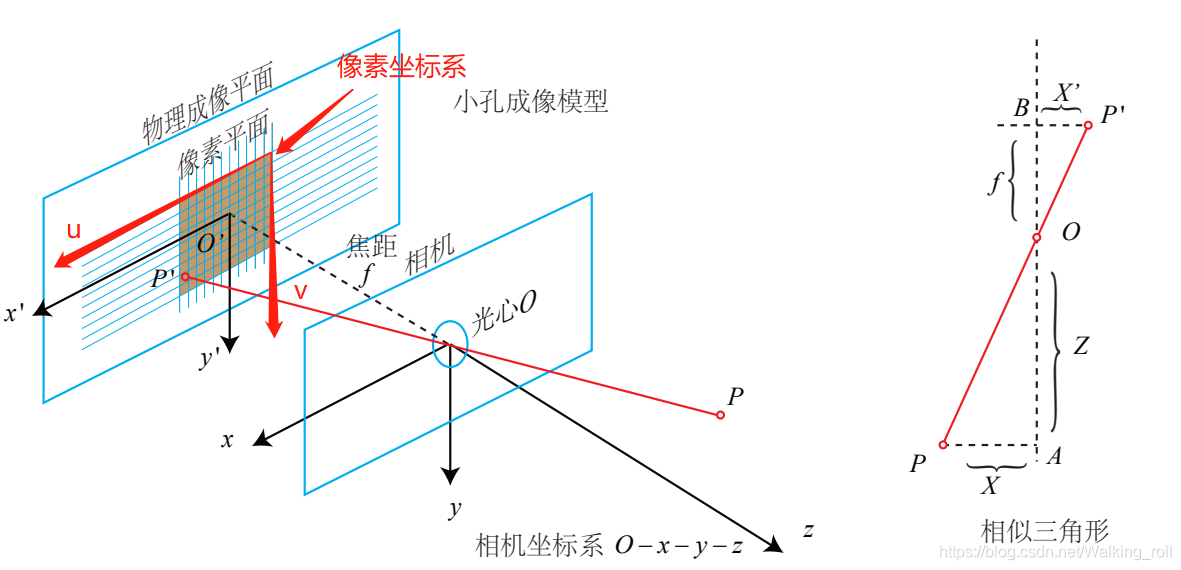
\includegraphics[width=0.5\textwidth]{figures/针孔相机.png}
\caption{针孔相机模型}
\end{figure}

这里我们定义两个坐标系:\textbf{图像坐标系}和\textbf{相机坐标系}。

具体定义方式为:图像坐标系的原点$O'$位于图像左上方,其$u$轴、$v$轴分别与$x'$,$y'$轴平行且方向相同。
像素坐标和成像平面之间,相差了缩放和平移的关系,这个关系可以用\textbf{线性变换}来表示。
我们设坐标在$u$轴上缩放了$\alpha$倍,在$v$轴上缩放了$\beta$倍,同时原点相对光轴平移了$[c_x,c_y]^T$。
则图像坐标系到相机坐标系的变换可以表示为:

\begin{equation}
\begin{cases}
    u = \alpha X' + c_x \\
    v = \beta Y' + c_y 
 \end{cases}
\end{equation}

根据初中学的小孔成像公式,带入镜头透镜x、y方向的焦距$f_x$、$f_y$,我们就可以得到:

\begin{equation}
    Z
    \begin{pmatrix}
        u \\ v \\ 1
    \end{pmatrix}
    =
    \begin{pmatrix}
        f_x & 0 & c_x \\
        0 & f_y & c_y \\
        0 & 0 & 1
    \end{pmatrix}
    \begin{pmatrix}
        X \\ Y \\ Z
    \end{pmatrix}
    \equiv K  P.
\end{equation}

我们把$K$称为\textbf{相机内参矩阵},内参是相机生产时刻确定的,与相机本身的特性无关。
同时$P$是相机在自身坐标系下的坐标,在真实情况下,我们通过世界坐标系来描述机器人的空间位姿,因此需要将$P$转换到相机坐标系。

其实,工程上使用的相机镜头是变化的,我们还需要进行标定获得更加准确的相机内参,但是本文假定已经完成了标定获得了准确的内参。

\begin{equation}
    Z P = Z 
    \begin{pmatrix}
        u\\v\\1
    \end{pmatrix}
    = K ( R P_{world} + t) = K T P_{world}
    \label{eq:rt}
\end{equation}

可以注意到,在相机的成像过程中我们将Z坐标归一化了,也就是失去了图像的深度信息,这对SLAM是十分致命的。
所以我们有两种路线解决这个问题:1、通过多个平面数据来源计算恢复深度信息;2、改进技术,使用能获得深度信息的相机。

\textbf{PnP就是一种选择第一个路线的算法}。

